\documentclass[10pt,conference,compsocconf]{IEEEtran}

\usepackage{hyperref}
\usepackage{graphicx}
\usepackage{amsmath}
\usepackage{booktabs}
\usepackage{xcolor}
\newcommand{\fillin}[1]{\textcolor{red}{#1}}

\begin{document}
\title{Predicting Coronary Heart Disease from Health Survey Data\\with Machine Learning Methods}

\author{
  \IEEEauthorblockN{Jibril Sakhoné}
  \IEEEauthorblockA{\textit{CS-433 Machine Learning, EPFL}\\
  jibril.sakhone@epfl.ch}
  \and
  \IEEEauthorblockN{Arnaud Lambelet}
  \IEEEauthorblockA{\textit{CS-433 Machine Learning, EPFL}\\
  arnaud.lambelet@epfl.ch}
}

\maketitle
\vspace{-4mm}

\begin{abstract}
We predict coronary heart disease (MICHD) from 321 answers of the 2015 BRFSS health survey.
Only 8.8\% of respondents are positive, so we optimise the F1 score by choosing the decision threshold that maximises it.
Starting from the six required regression methods, we show that the largest single gain comes from training logistic regression to convergence with Newton's method.
Data cleaning, interaction features and two non-linear models (a neural network and gradient-boosted trees) add smaller gains.
Averaging the three models reaches an out-of-fold F1 of \textbf{0.4345} in cross-validation (vs.\ 0.419 for the best required method) and an F1 of 0.446 on the AIcrowd test set.
All methods are implemented from scratch in NumPy.
\end{abstract}

\section{Introduction}
Cardiovascular diseases are one of the leading causes of death worldwide, and predicting them early is an important challenge.
Machine learning can find patterns in health and lifestyle data that help predict this risk.
We address a binary classification task: predicting whether a person has reported a history of myocardial infarction or coronary heart disease (MICHD) from their answers to the Behavioral Risk Factor Surveillance System (BRFSS), a U.S. telephone survey on health behaviours, chronic conditions and preventive care.
We compare several approaches with local cross-validation, to measure the impact of preprocessing and modelling choices and to understand their limitations.

\section{Models and Methods}

\subsection{Data cleaning and features}
\begin{enumerate}
\item \textbf{Survey codes.} In BRFSS, 7/9, 77/99, 777/999 mean ``don't know''/``refused''; we set them to missing. Codes 88/888 mean ``none'' and become 0. The codes are inferred from each column's maximum value.
\item \textbf{Codebook decoding.} Some columns mix units, e.g.\ weight in pounds (50--776) or kilograms ($9000+$kg), or fruit intake coded as $1xx$ per day, $2xx$ per week, $3xx$ per month. We convert 14 such columns to one unit.
\item \textbf{Column selection.} We drop 19 columns describing the survey itself (date, state, sampling weights) and columns more than 90\% missing.
\item \textbf{Encoding.} Answers with $\le 10$ distinct values are one-hot encoded, with a ``missing'' level. Numeric answers get $\log(1+x)$ if strongly skewed (skewness $>2$), then median imputation and standardisation. A bias column is added, giving 483 features.
\end{enumerate}
All statistics (medians, means, categories) are computed on the training data only.

\subsection{Choosing the decision threshold}
Every model outputs a score $s(x)$ (a probability for logistic models).
We predict MICHD if $s(x)\ge t$.
F1 is not differentiable, so instead of optimising it directly we train with a smooth loss and pick the $t$ that maximises F1 on the training folds.
This is how we handle the class imbalance (Fig.~\ref{fig:threshold}); re-weighting the positive class in the loss did not help (Table~\ref{tab:other}).

\begin{figure}[tbp]
  \centering
  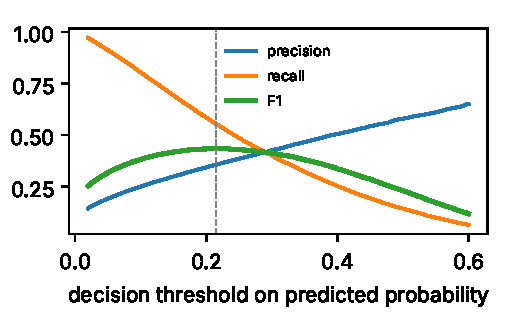
\includegraphics[width=0.62\columnwidth]{threshold}
  \vspace{-3mm}
  \caption{Precision, recall and F1 of the final model versus the threshold $t$ (out-of-fold predictions). The default $t=0.5$ gives F1 0.23 (2\% predicted positive); the best $t=0.215$ gives F1 0.4345 (14\% predicted positive).}
  \label{fig:threshold}
  \vspace{-3mm}
\end{figure}

\subsection{Baselines: the six required methods}
We use the methods of \texttt{implementations.py} with labels $y\in\{0,1\}$ on the basic features (columns $\le 50\%$ missing, no codebook, 358 features).
For gradient descent (GD) the step size must satisfy $\gamma<2/L$, where $L=33.8$ is the largest eigenvalue of $X^\top X/N$; larger steps diverged.
We use $\gamma=1/L=0.03$ for the MSE and $\gamma=4/L\approx0.1$ for the logistic loss (whose curvature is at most $L/4$), with 1000 iterations.
SGD uses 20,000 single-sample steps with $\gamma=10^{-3}$, and ridge and regularised logistic regression use $\lambda=10^{-4}$.
Because some BRFSS variables are exact functions of others, $X^\top X$ is singular, so for least squares we use the minimum-norm solution (pseudo-inverse).

\subsection{Our three models}
\textbf{A. Logistic regression with Newton's method.}
We minimise $\frac1N\sum_n[\log(1+e^{x_n^\top w})-y_n x_n^\top w]+\lambda\|w\|^2$ with Newton steps
$w\leftarrow w-\eta H^{-1}\nabla L$, where $H=X^\top S X/N+2\lambda I$ and $S=\mathrm{diag}(p_n(1-p_n))$.
The step $\eta$ is halved until the loss decreases.
This converges in about 7 iterations, whereas GD is still far from the optimum after 1000 iterations.
We add the pairwise products of the 20 features most correlated with the label (190 new features, chosen inside each training fold); $\lambda=10^{-4}$.

\textbf{B. Neural network.}
A multi-layer perceptron (483--128--64--1, ReLU) is trained on the logistic loss with Adam (learning rate $5\cdot10^{-4}$, batch 512, 6 epochs, weight decay $10^{-4}$).
We average 3 networks with different random seeds.

\textbf{C. Gradient-boosted trees.}
Each of 300 trees (depth 5) fits the second-order Taylor expansion of the logistic loss, as in XGBoost.
A split is chosen by the gain $\frac{G_L^2}{H_L+\lambda}+\frac{G_R^2}{H_R+\lambda}-\frac{G^2}{H+\lambda}$, where $G,H$ are sums of gradients and Hessians.
Each leaf predicts $-0.1\,G/(H+\lambda)$.
Features are binned into 32 quantile bins, with missing values in their own bin, so no imputation is needed.
Each tree sees a random half of the rows and features.


\subsection{Evaluation}
We use stratified 5-fold CV (same positive rate in every fold, fixed seed).
The threshold is tuned on the 4 training folds and F1 is measured on the 5th; we report the mean $\pm$ standard deviation over folds.
Feature selection and interactions use the labels, so they are computed inside each training fold.
The final prediction averages the probabilities of A, B and C; its threshold maximises F1 on all out-of-fold predictions (OOF-F1).

\section{Results}

\begin{table}[tbp]
\centering
\caption{The six required methods (basic features, 5-fold CV).}
\label{tab:baselines}
\begin{tabular}{lcc}
\toprule
Method & F1 & Accuracy\\
\midrule
GD, MSE ($\gamma$=0.03) & 0.4176 $\pm$ .005 & 0.868\\
SGD, MSE ($\gamma$=$10^{-3}$) & 0.3519 $\pm$ .047 & 0.840\\
Least squares & 0.4178 $\pm$ .005 & 0.868\\
Ridge regression & 0.4167 $\pm$ .005 & 0.864\\
Logistic regression, GD & 0.4189 $\pm$ .003 & 0.869\\
Reg.\ logistic regression, GD & 0.4193 $\pm$ .003 & 0.868\\
\bottomrule
\end{tabular}
\vspace{-2mm}
\end{table}

\begin{table}[tbp]
\centering
\caption{Ablation, one change at a time (std $\approx$0.004).}
\label{tab:ablation}
\begin{tabular}{lcc}
\toprule
Step & F1 & OOF-F1\\
\midrule
I.6\ \ Reg.\ logistic, GD (best of Table~\ref{tab:baselines}) & 0.4193 & 0.4193\\
II.1\ Newton's method (converged) & 0.4278 & 0.4279\\
II.2\ + keep columns $\le$90\% missing & 0.4283 & 0.4296\\
II.3\ + codebook decoding + log & 0.4296 & 0.4305\\
II.4\ + interactions = \textbf{model A} & 0.4308 & 0.4311\\
\midrule
II.5\ Neural networks = \textbf{model B} & 0.4303 & 0.4316\\
II.6\ Boosted trees = \textbf{model C} & 0.4273 & 0.4313\\
\midrule
Average A + B & -- & 0.4327\\
Average A + C / B + C & -- & 0.4339 / 0.4341\\
\textbf{Average A + B + C (final)} & -- & \textbf{0.4345}\\
\bottomrule
\end{tabular}
\vspace{-2mm}
\end{table}

\begin{table}[tbp]
\centering
\caption{Ideas that did not help (model of II.3).}
\label{tab:other}
\begin{tabular}{lcc}
\toprule
Variant & F1 & OOF-F1\\
\midrule
Class weight 10 for positives & 0.4283 & 0.4299\\
Feature selection (top 200 by correlation) & 0.4241 & 0.4245\\
Add squared numeric features & 0.4301 & 0.4308\\
No one-hot encoding (raw codes) & 0.4253 & 0.4265\\
\bottomrule
\end{tabular}
\vspace{-3mm}
\end{table}

\textbf{Baselines (Table~\ref{tab:baselines}).}
All linear methods reach F1 $\approx$0.418.
GD on the MSE matches the closed-form least-squares solution, so it has converged.
SGD with single-sample steps is much noisier (std 0.047).
Logistic GD (0.419) is only slightly better, as it has not converged (see II.1).

\textbf{Ablation (Table~\ref{tab:ablation}).}
Solving the same logistic regression to convergence with Newton's method is the largest single gain (+0.009).
Keeping more columns, decoding the codebook and adding interactions each add about 0.001.
The neural network and the trees are no better than model A alone.
Averaging them, however, raises the out-of-fold F1 to 0.4345, because the three models make different errors.
In total, F1 improves from 0.419 to 0.4345 (+0.015).

\textbf{Test set.} Our first submission (logistic GD, CV F1 0.4245) scored F1 0.437 and accuracy 0.877 on AIcrowd.
The final model scores F1 0.446 and accuracy 0.878.

\textbf{What did not help (Table~\ref{tab:other}).}
Up-weighting the positives changes nothing once the threshold is tuned: both shift the decision towards the rare class.
Keeping only the 200 features most correlated with the label hurts ($-$0.006), since the L2 penalty already shrinks weak features while dropped ones still carry information.
Removing one-hot encoding costs 0.004, showing that the survey codes are categories, not ordered numbers.

\section{Discussion}
With a fold-to-fold standard deviation of about 0.004, changes below $\approx$0.002 are not meaningful.
The clearest effects come from optimisation (convergence) and model combination; feature engineering mattered less than expected.
Most of the signal seems roughly linear in well-encoded features, and the remaining errors differ between model types.

\textbf{Limitations.}
Label-free preprocessing is fit on the whole training set before CV (no label leakage).
The final OOF-F1 uses a threshold tuned on the same predictions, so it is slightly optimistic.

\textbf{Summary.}
Tuning the threshold for F1 handled the class imbalance, converging logistic regression with Newton's method gave the largest gain, and averaging three different models gave the best out-of-fold F1 (0.4345).

\textbf{Use of AI.} We used an AI assistant (Claude) to help write a few function definitions and this report.



\end{document}
